\chapter{提案手法}
\label{chap:design}

本章では、本研究の目的を達成するための手法とその設計を示す。

\section{概要}

本論文で提案する手法では、糖尿病患者のインスリン摂取忘れを検知するために以下の2つのイベントが起こった時間を用いり、
これらを活用することで、患者がインスリンを打ち忘れた際に通知をすることを目指す。

\begin{enumerate}
  \item インスリンペンを使用してインスリンが摂取された時間
  \item 患者本人が食事を開始した時間
\end{enumerate}

インスリンペンを使用してインスリンが摂取された時間は、インスリン自体が摂取されたことを図るのに必要になるが、これは2番目の食事を開始した時間と比較して食前にインスリンが摂取されたかどうかを判別するための重要なデータとなる。
食事を開始した時間については今述べたようにインスリンが摂取された時間との比較に使うが、この食事というイベントの時間を利用することで、固定時間式のリマインダーなどよりも即時性が高くなる。
患者は、もし打ち忘れたことを食事中、ないし食事終了直後に気づくことができた場合、通常通りインスリンを打てば良いとされており、\cite{insulin_qa_sakaemachi_nishi} \cite{insulin_qa_akaike}
さらに後になって気付いた場合には、担当医と連絡を取り、指示を仰いだ上で正確な対処を自分で行わなければならない。\cite{insulin_qa_senior}
糖尿病患者にとっての負担を減らすためにも、この即時性は重要な点であるため、今回、この食事というイベント駆動の手法を提案した。

そしてこれら2つの時間データを取得するためには以下の2つのデバイスが必要になる。

\begin{enumerate}
  \item インスリンペンに装着し、インスリンが投与されたことを検知、その時間を取得するデバイス
  \item 食卓上に設置され、食事開始を検知し、その時間を取得するデバイス
\end{enumerate}

今回の実装では、(インスリンペンに装着するデバイス(短い、かつはっきりと何を指しているかわかる名前に置き換える))は時間を取得した後、独自のWebサーバーにその検知時間をアップロードする。
これによりWebサーバーを通じてデータベースにその時間が記録される。
そして2の(食事開始を検知し、その時間を取得するデバイス(短い、かつはっきりと何を指しているかわかる名前に置き換える))は、その時間が取得された際に、データベースに記録された直近のインスリン摂取時間を確認、比較する。
比較した結果、そのインスリン摂取時間が食事開始時間よりも前で、さらにその差が所定の時間以内だった場合はインスリンは正常に摂取されたと判定し、
そうでなかった場合にはインスリン摂取は行われず、患者は打ち忘れていると判定し通知を行う。

図\ref{fig:insulin_design}にその概要とフローを示す。

\begin{figure}[htbp]
  \caption{インスリン摂取忘れ検知の概要とフロー}
  \label{fig:insulin_design}
  \begin{center}
    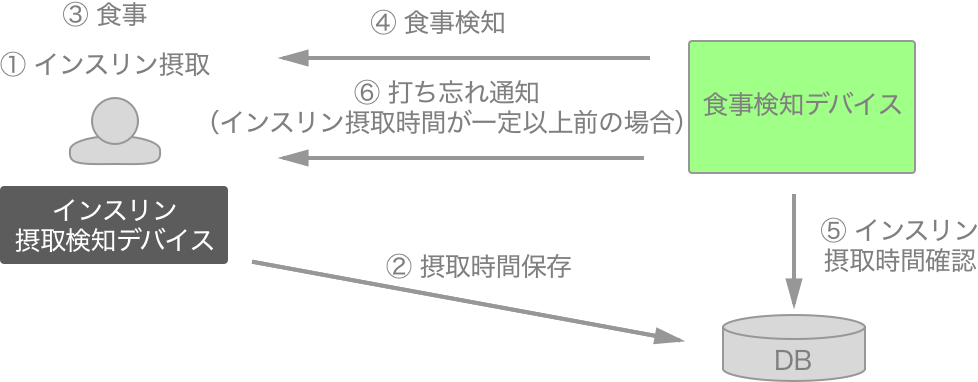
\includegraphics[bb=0 0 1000 530,width=15cm]{assets/insulin_design.png}
  \end{center}
\end{figure}

\section{インスリン摂取の検知方法}

糖尿病患者がインスリンペンを使ってインスリンを摂取する際は、自分に必要なだけの量を摂取するためにペンの端の目盛りを回して調節し、
下腹部に針を刺した状態でゆっくりとペンの端を押していく(図\ref{fig:insulin_pen_push}を参照)。本論文では、このインスリンペンの端を指で押す、というイベントに着目して摂取の判定に利用した。
指で押されるということは、そこに圧力が加わるので、タクタイルスイッチ\cite{tactile_switch}と同じ仕組みを利用することで、これを引き金に摂取時間を取得アップロードすることができる。
本研究では、この手法を実装したスイッチをインスリンペンの端、つまりインスリン摂取の際に押下される位置にこのデバイスを取り付けることで検知することを目指す。

\begin{figure}[htbp]
  \caption{インスリンの押下部}
  \label{fig:insulin_pen_push}
  \begin{center}
    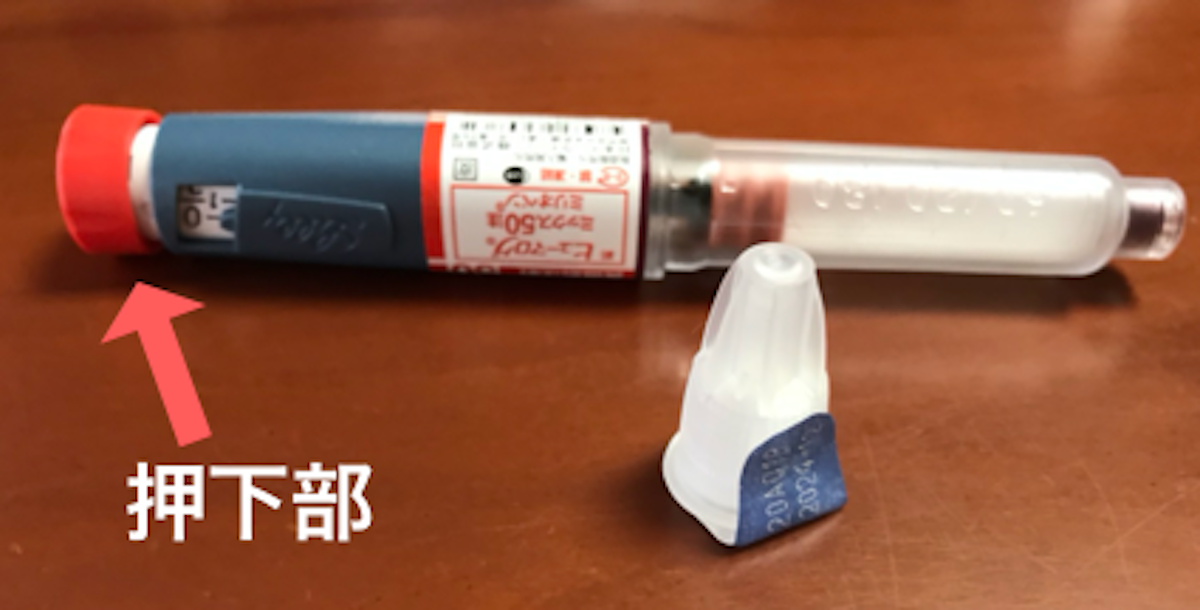
\includegraphics[bb=0 0 1300 1000,width=10cm]{assets/insulin_pen_push.png}
  \end{center}
\end{figure}

\section{食事行動の検知方法}

重さがある物体が机の上に置かれた時、重量によって大小様々ではあるが机に振動が起きる。そして食卓は、コップ、食器、スマホなど日常生活の中で様々な物体が置かれる場所であり、
さらに物が置かれる他にも、人間が作業をしたりなど様々な活動が行われる場所である。
そこで、本研究ではこの振動に着目し、食事中も食器を置く際の振動の振幅の大きさと、パターンから食事行動が検知できるのではないかと仮説をたてた。
本研究の提案手法がそもそも食事検知を達成し得る手法であるのかを検証すべく、以下の場面で振動データを計測、収集、比較し、食事時もしくは食器を置く時の振動がどれくらい特徴的なのかを調べた。

%動作のリスト
\begin{enumerate}
  \item コップを置いた時
  \item 茶碗を置いた時
  \item ノートパソコンでタイピングをした時(Helloworldの文字を入力)
  \item 携帯を置いた時
\end{enumerate}

動作の振動データを取得する際に用いたのは、以下のアイテムである。

\begin{itemize}
  \item 水の入ったコップ - 約600g
  \item ご飯の入った茶碗 - 約300g
  \item Macbook Pro 13 inch
  \item iFaceカバー付きiPhone XS - 約270g
\end{itemize}

図\ref{fig:actions_vibration}に、それぞれの振動データとその動作が行われた時点を示しているが、茶碗を置いた時、iPhoneを置いた時などは振幅が大きく、
机に大きな振動が伝わったことがわかった。一方で、コップが置かれた時、ノートパソコンのタイピング時は明らかに振動が少なく、振れ幅が大きくないようであった。

\begin{figure}[htbp]
  \caption{それぞれの動作の振動データ}
  \label{fig:actions_vibration}
  \begin{center}
    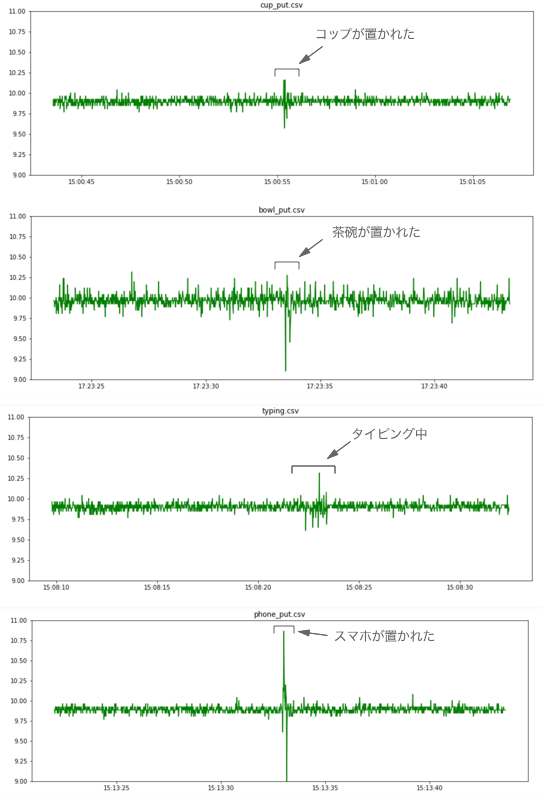
\includegraphics[bb=0 0 700 800,width=20cm]{assets/actions_vibration.png}
  \end{center}
\end{figure}

この実験から、動作により振幅が変化することがわかった。しかしながら、単体の動作の振動のみでは何が置かれたか、どのような動作をしているのかは判別が難しい。
食事をしている最中は皿を持ち変えるため、皿を置くという動作がある一定期間に複数回行われる。また、ノートパソコンで作業している時は入力やクリック動作が連続的に行われるため、振動にある一定のパターンが生まれる。
そして、この一連の連続的な動作からどれくらいそれぞれの活動の特徴が見出せるのかを実験した。
以下の活動から、一定期間分の振動データを取得して比較を行った。
今回の実験で取得したデータは以下の活動である。

%活動のリスト
\begin{enumerate}
  \item 食事中
  \item ノートパソコンでの作業中
  \item 部屋内で運動中
\end{enumerate}

図\ref{fig:activities_vibration}がノートパソコンでの作業中と部屋内で運動中に机に与えられた振動のデータである。
そして図\ref{fig:meal_vibration}が食事中に起きる振動のデータである。3つのどれも、ある程度特徴が見られたが、
食事中は、今回の測定時の平均加速度で約10\si{m/s^{2}}から、おおよそ誤差0.75\si{m/s^{2}}以上、2\si{m/s^{2}}以下の単発の振動が一定周期で起きており、
食事イベントを判定するには十分な特徴が見て取れた。

このデータに加えてさらに、20代男性3人の協力を得て、自分を含め合計4人のデータをもとに食事検知のためのアルゴリズムを組んだ。
この4人のデータをもとに組んだアルゴリズムは以下である。

\begin{enumerate}
  \item 平均加速度から上下誤差0.65\si{m/s^{2}}より大きく、2\si{m/s^{2}}未満の場合これを食器が置かれたものと判定する。
  \item 500ms以内に起こった1を満たす複数の振動は、単一のものを置いた際に起こった余振動とする。よってこれはまとめて1回と見なす。
  \item 2\si{m/s^2}を超える振動が起こり、その後500ms以内に起こった1を満たす複数の振動は、食器以外の単一のものを置いた際に起こった余振動とする。よってこれはカウントしない。
  \item 500ms以降、1500ms以内に起こった1を満たす振動が検知された場合、これを食器以外の何かが置かれた、もしくは何か他の動作が行われているとして、0.2回分カウントを減らし、食事であるという判定から遠ざかる。
  \item 1を満たす振動が2分以内の感覚で、連続6回検知された場合、これを食事として検知する。
  \item 2分以上1を満たす振動が起きなかった場合は、カウントをリセットし、その一連の振動は食事によるものではないと判断する。
\end{enumerate}

\begin{figure}[htbp]
  \caption{それぞれの一連の動作から取得した振動データ}
  \label{fig:activities_vibration}
  \begin{center}
    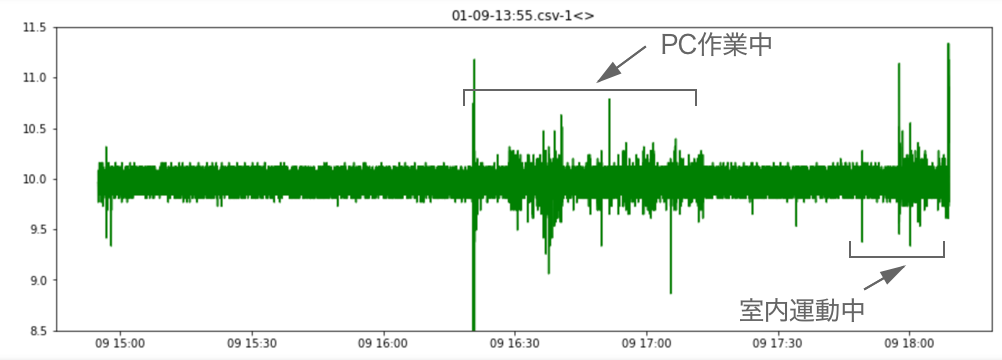
\includegraphics[bb=0 0 1200 300,width=20cm]{assets/pc_task_n_exercise.png}
  \end{center}
\end{figure}

\begin{figure}[htbp]
  \caption{食事中の振動データ}
  \label{fig:activities_vibration}
  \begin{center}
    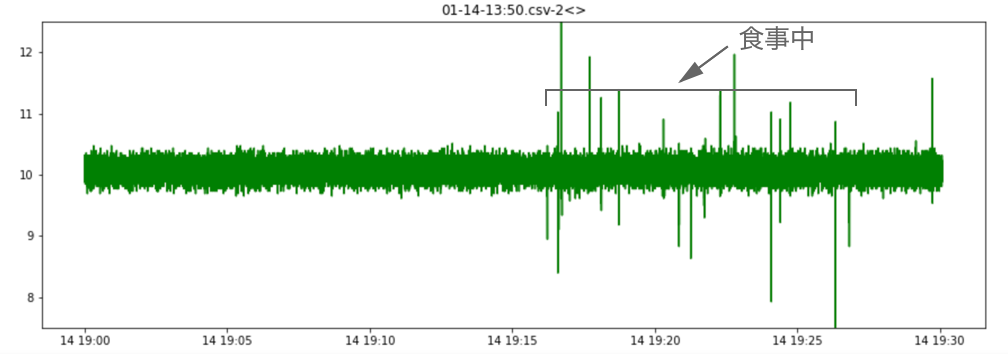
\includegraphics[bb=0 0 1200 300,width=20cm]{assets/meal_vibration.png}
  \end{center}
\end{figure}

\section{インスリン摂取忘れの通知}

インスリン忘れの通知にはスピーカーを使用した音声通知を利用する。
食事検知が行われた時、その食事が検知された時間から直近30分以内にインスリン摂取が確認できなかった場合、これをインスリン摂取忘れとし、通知を行う。


